\documentclass{article}

\usepackage{tikz}

\begin{document}

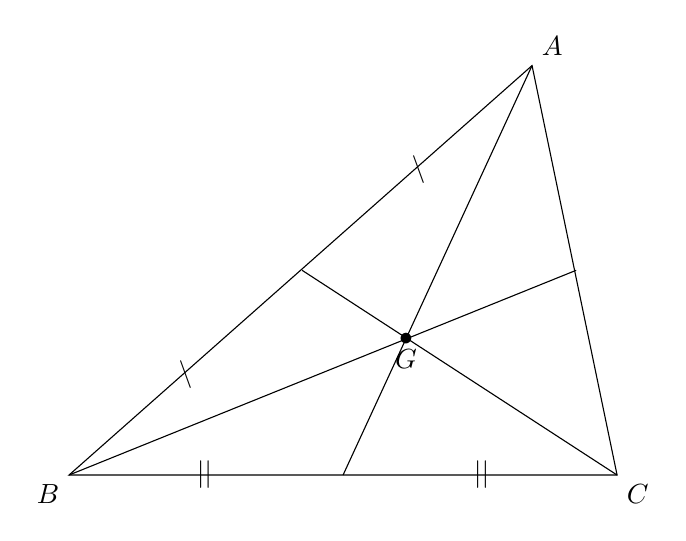
\begin{tikzpicture}[scale=4]
  \draw % triangle
     (0.87,-0.5) node[below right]{$C$}
     -- (0.6,0.8) node[above right]{$A$} 
     -- (-0.87,-0.5) node[below left]{$B$}
     -- cycle ;
  \draw  % medianes
     (0.6,0.8) -- (0,-0.5) % mediane issue de A
     (-0.87,-0.5) -- (0.74, 0.15) % mediane issue de B
     (0.87,-0.5) -- (-0.13, 0.15); % mediane issue de C
  \draw (0.2,-0.07) node{$\bullet$} node[below] {$G$}; % centre
  % marques
  \draw (0.24, 0.47) node {\textbackslash}; % marque sur [AB], vers A
  \draw (-0.5, -0.18) node {\textbackslash};  % marque sur [AB], vers B    
  \draw (-0.44, -0.5) node{$||$} ; % marque sur [BC], vers B
  \draw (0.44, -0.5) node{$||$} ; % marque sur [BC], vers C
\end{tikzpicture}

\end{document}
